\documentclass[SingleSpace,12pt,Proceedings]{Serre_ASCE}

\usepackage[dvips]{graphicx}
\usepackage{amsmath}
\usepackage{amsfonts}
\usepackage{amssymb}
\usepackage[pdf]{pstricks}
\usepackage{psfrag}
\usepackage{pifont}
\usepackage{epstopdf}
%\usepackage{topcapt}
\usepackage{lscape}
\usepackage{amsthm}
\usepackage{url}
\usepackage{pifont}
\usepackage{geometry}
\usepackage{fleqn}
\usepackage{txfonts}
\usepackage{wasysym}
\usepackage{lineno}
\usepackage{enumerate}
\usepackage{url}
\usepackage{times}
\usepackage{subfigure}
\usepackage{graphicx}
\usepackage{longtable}
%\usepackage{citeref}
\usepackage[skip=0pt]{caption}

% TIME ON EVERY PAGE AS WELL AS THE FILE NAME
\usepackage{fancyhdr}
\usepackage{currfile}
\usepackage[us,12hr]{datetime} % `us' makes \today behave as usual in TeX/LaTeX
\fancypagestyle{plain}{
\fancyhf{}
\rfoot{\small Draft Paper \\ File Name: {\currfilename} \\ Date: {\ddmmyyyydate\today} at \currenttime}
\lfoot{Page \thepage}
\renewcommand{\headrulewidth}{0pt}}
\pagestyle{plain}

\begin{document}

\title{Behaviour of the Dam-Break Problem for the Serre Equations}

\author{
Jordan~Pitt,%
\thanks{Mathematical Sciences Institute, Australian National University, Canberra, ACT 0200, Australia, E-mail: Jordan.Pitt@anu.edu.au. The work undertaken by the first author was supported financially by an Australian National University Scholarship.}
\\
Christopher~Zoppou,\footnotemark[1]%
%
% Adding a second author with the same affiliation (still using \thanks):
\\
Stephen~G.~Roberts,\footnotemark[1]
}

\maketitle

\begin{abstract}

\end{abstract}

\KeyWords{dispersive waves, conservation laws, Serre equation, finite volume method, finite difference method}

\linenumbers

%--------------------------------------------------------------------------------
\section{Introduction} \label{intro} 

%--------------------------------------------------------------------------------
\section{Serre Equations}
\label{section:Serre Equations}
The Serre equations can derived as an approximation to the full Euler equations by depth integration similar to \cite{Su-Gardener-1969-536}. They can also be seen as an asymptotic expansion to the Euler equations as well \cite{Bonneton-Lannes-2009-16601}. The former is more consistent with the perspective from which numerical methods will be developed while the latter indicates the appropriate regions in which to use these equations as a model for fluid flow.
\begin{figure}[htb]
\begin{center}
\includegraphics[width=7.0cm]{one-dimensional-axis_Serre.eps}
\end{center}
\caption{The notation used for one-dimensional flow governed by the Serre equation.}
\label{fig:Notation}
\end{figure}
The set up of the scenario under which the Serre approximation is made consists of a two dimensional $\textbf{x} = (x,z)$ fluid over a bottom topography as in Figure \ref{fig:Notation} acting under gravity. Consider a fluid particle at depth  $\xi(\textbf{x},t) = z - h(x,t) - z_b(x)$ below the water surface, see Figure \ref{fig:Notation}. Where the water depth is $h(x,t)$ and $z_b(x)$ is the bed elevation. The fluid particle is subject to the pressure, $p(\textbf{x},t)$ and  gravitational acceleration, $\textbf{g} = (0,g)^T$ and has a velocity $\textbf{u} = (u(\textbf{x},t),w(\textbf{x},t))$,  where $u(\textbf{x},t)$ is the velocity in the $x$-coordinate and $w(\textbf{x},t)$ is the velocity in the $z$-coordinate and $t$ is time. Assuming that $z_b(x)$ is constant the Serre equations read \cite{Guyenne-etal-2014-169}
\begin{linenomath*}
\begin{subequations}\label{eq:Serre_conservative_form}
\begin{gather}
\dfrac{\partial h}{\partial t} + \dfrac{\partial (\bar{u}h)}{\partial x} = 0
\label{eq:Serre_continuity}
\end{gather}
\begin{gather}
\underbrace{\underbrace{\dfrac{\partial (\bar{u}h)}{\partial t} + \dfrac{\partial}{\partial x} \left ( \bar{u}^2h + \dfrac{gh^2}{2}\right )}_{\text{Shallow Water Wave Equations}} + \underbrace{\dfrac{\partial}{\partial x} \left (  \dfrac{h^3}{3} \left [ \dfrac{\partial \bar{u} }{\partial x} \dfrac{\partial \bar{u}}{\partial x} - \bar{u} \dfrac{\partial^2 \bar{u}}{\partial x^2}  - \dfrac{\partial^2 \bar{u}}{\partial x \partial t}\right ] \right )}_{\text{Dispersion Terms}} = 0.}_{\text{Serre Equations}}
\label{eq:Serre_momentum}
\end{gather}
\end{subequations}
\end{linenomath*}
Where $\bar{u}$ means the average of $u$ over the depth of water.
%--------------------------------------------------------------------------------
%--------------------------------------------------------------------------------
\section{Finite Difference and Lax Wendroff}
\label{section:}
This method was used in \citeN{El-etal-2006} for the Serre equations. It consists of a lax-wendroff update for $h$ and a spatio-temporal second order approximation to [] which results in a fully second-order method. To make this method precise it will be presented here in sufficient replicable detail.

Note that [] is in conservative law form for $h$ where the Jacobian is $u$, where the bar has been dropped to simplify the notation. Thus assuming a fixed resolution discretisation for space and time which will be represented as follows $q^n_i = q(x_i,t^n)$ for some quantity $q$ the lax-wendroff update for $h$ obtained is
\begin{linenomath*}
\begin{gather}
\begin{split}
h^{n+1}_i &= h^{n}_i - \frac{\Delta t}{2\Delta x} \left(\left(uh\right)^n_{i+1} - \left(uh\right)^n_{i-1}\right) \\ &+ \frac{\Delta t^2}{2\Delta x^2}\left(\frac{u^n_{i+1} - u^n_{i} }{2}\left(\left(uh\right)^n_{i+1} - \left(uh\right)^n_{i}\right) - \frac{u^n_{i} - u^n_{i-1} }{2}\left(\left(uh\right)^n_{i} - \left(uh\right)^n_{i-1}\right) \right)
\end{split}
\label{eq:LW4h}
\end{gather}
\end{linenomath*}

To get a second-order approximation to [] is built by first expanding all the derivatives out and making use of the continuity equation [], this results in:
\begin{linenomath*}
\begin{subequations}
\begin{gather}
h\dfrac{\partial u}{\partial t} + X - h^2\frac{\partial^2 u}{\partial x \partial t} - \frac{h^3}{3}\frac{\partial^3 u}{\partial x^2 \partial t}  =0 
\label{eq:expandedu}
\end{gather}
where $X$ contains only spatial derivatives and is
\begin{gather}
X = uh\frac{\partial u}{\partial x} + gh\frac{\partial h}{\partial x} + h^2\frac{\partial u}{\partial x}\frac{\partial u}{\partial x} + \frac{h^3}{3}\frac{\partial u}{\partial x}\frac{\partial^2 u}{\partial x^2} - h^2u\frac{\partial^2 u}{\partial x^2}- \frac{h^3}{3}u\frac{\partial^3 u}{\partial x^3} .
\end{gather}
\end{subequations}
\end{linenomath*}
Then taking second-order approximations to the time derivatives for [] gives
\begin{linenomath*}
\begin{gather}
h^{n}\dfrac{u^{n+1} - u^{n-1}}{2 \Delta t} + X^{n} - \left(h^{n}\right)^2\frac{ \left(\frac{\partial u}{\partial x}\right)^{n+1} - \left(\frac{\partial u}{\partial x}\right)^{n-1} }{2 \Delta t} - \frac{\left(h^{n}\right)^3}{3}\frac{ \left(\frac{\partial^2 u}{\partial x^2}\right)^{n+1} - \left(\frac{\partial^2 u}{\partial x^2}\right)^{n-1} }{2 \Delta t}  =0 
\label{eq:expandedutdisc}
\end{gather}
\end{linenomath*}
\begin{linenomath*}
\begin{gather}
h^{n} \left(u^{n+1} - u^{n-1}\right) + 2\Delta tX^{n} - \left(h^{n}\right)^2 \left(\left(\frac{\partial u}{\partial x}\right)^{n+1} - \left(\frac{\partial u}{\partial x}\right)^{n-1}\right) - \frac{\left(h^{n}\right)^3}{3}\left(\left(\frac{\partial^2 u}{\partial x^2}\right)^{n+1} - \left(\frac{\partial^2 u}{\partial x^2}\right)^{n-1} \right)  =0 
\label{eq:expandedutdisc1}
\end{gather}
\end{linenomath*}

\begin{linenomath*}
\begin{gather}
h^{n}u^{n+1} - \left(h^{n}\right)^2 \left(\frac{\partial u}{\partial x}\right)^{n+1} - \frac{\left(h^{n}\right)^3}{3}\left(\frac{\partial^2 u}{\partial x^2}\right)^{n+1}  + 2\Delta tX^{n} - h^{n}u^{n-1} + \left(h^{n}\right)^2\left(\frac{\partial u}{\partial x}\right)^{n-1} + \frac{\left(h^{n}\right)^3}{3}\left(\frac{\partial^2 u}{\partial x^2}\right)^{n-1}   =0 
\label{eq:expandedutdisc2}
\end{gather}
\end{linenomath*}
Let
\begin{linenomath*}
\begin{gather}
Y^n = 2\Delta tX^{n} - h^{n}u^{n-1} + \left(h^{n}\right)^2\left(\frac{\partial u}{\partial x}\right)^{n-1} + \frac{\left(h^{n}\right)^3}{3}\left(\frac{\partial^2 u}{\partial x^2}\right)^{n-1}
\label{eq:expandfactor Xp}
\end{gather}
\end{linenomath*}

Taking second-order approximations to the spatial derivatives gives
\begin{linenomath*}
\begin{gather}
h^{n}_iu^{n+1}_i - \left(h^{n}_i\right)^2 \left(\frac{u^{n+1}_{i+1} -u^{n+1}_{i-1} }{2 \Delta x}\right) - \frac{\left(h^{n}_i\right)^3}{3}\left(\frac{u^{n+1}_{i+1} - 2u^{n+1}_{i} + u^{n+1}_{i-1} }{\Delta x^2}\right) = - Y^n_i 
\label{eq:expandedutdisc3}
\end{gather}
\end{linenomath*}
This can be rearranged into a tri-diagonal matrix that updates $u$ given its current and previous values. So that
\begin{linenomath*}
\begin{gather*}
\left[\begin{array}{c}
 u^{n+1}_0 \\
 \vdots \\
 u^{n+1}_m \end{array}\right]
 = A^{-1} \left[\begin{array}{c}
  -Y^n_0 \\
  \vdots \\
  -Y^n_m \end{array}\right] =: \mathcal{G}_u\left(\boldsymbol{u}^n,\boldsymbol{h}^n, \boldsymbol{u}^{n-1}, \Delta t \right).
\end{gather*}
\end{linenomath*}
Where
\begin{linenomath*}
\begin{gather*}
A =
\left[\begin{array}{ccccccccc}
 b_0 & c_0 &  & & & &  \\
 a_0 & b_1 & c_1 &  & & & \\
  & a_1 & b_2 & c_2 &  & &   \\
  &  &\ddots &\ddots &\ddots & & \\
  &  &  & a_{m-3} & b_{m-2} & c_{m-2} & \\
  &  &  &  & a_{m-2} & b_{m-1} & c_{m-1} \\
  &  &  & &  & a_{m-1} & b_{m}\\
  \end{array}\right]
\end{gather*}
\end{linenomath*}
with
\begin{subequations}
\begin{gather}
a_{i-1} = \frac{\left(h^n_i\right)^2}{2\Delta x}\frac{h^n_{i+1} - h^n_{i-1}}{2\Delta x} - \frac{\left(h^n_i\right)^3}{3 \Delta x^2}  ,
\label{eq:utriAa}
\end{gather}
\begin{gather}
b_i = h^n_i + \frac{2 h^n_i}{3 \Delta x^2}
\label{eq:utriAb}
\end{gather}
and
\begin{gather}
c_i = -\frac{\left(h^n_i\right)^2}{2\Delta x}\frac{h^n_{i+1} - h^n_{i-1}}{2\Delta x} - \frac{\left(h^n_i\right)^3}{3 \Delta x^2}.
\label{eq:utriAc}
\end{gather}
\end{subequations}
Lastly the final expression for $Y^n_i$ is given by:

\begin{linenomath*}
\begin{gather}
\begin{split}
Y^n_i = 2\Delta tX_i^{n} - h_i^{n}u_i^{n-1} + \left(h_i^{n}\right)^2\frac{u^{n-1}_{i+1} - u^{n-1}_{i-1}}{2\Delta x} + \frac{\left(h_i^{n}\right)^3}{3}\frac{u^{n-1}_{i+1} -2 u^{n-1}_{i} + u^{n-1}_{i-1}}{\Delta x^2}
\end{split}
\end{gather}
\end{linenomath*}

\begin{linenomath*}
\begin{gather}
\begin{split}
Y^n_i &= 2\Delta t \Bigg[u^n_ih^n_i \frac{u^{n}_{i+1} - u^{n}_{i-1}}{2\Delta x} + gh^n_i\frac{h^{n-1}_{i+1} - h^{n-1}_{i-1}}{2\Delta x} + \left(h^n_i\right)^2 \left(\frac{u^{n-1}_{i+1} - u^{n-1}_{i-1}}{2\Delta x} \right)^2 \\ &+ \frac{\left(h^n_i\right)^3}{3}\frac{u^{n}_{i+1} - u^{n}_{i-1}}{2\Delta x}\frac{u^{n}_{i+1} -2u^{n}_{i}   + u^{n}_{i-1}}{\Delta x^2} - \left(h^n_i\right)^2u^n_i\frac{u^{n}_{i+1} -2u^{n}_{i} + u^{n}_{i-1}}{\Delta x^2}  \\  &- \frac{\left(h^n_i\right)^3}{3}u^n_i\frac{ u^n_{j+2} - 2u^n_{j+1} + 2 u^n_{j-1} - u^n_{j-2}}{2 \Delta x^3} \Bigg] \\ &- h_i^{n}u_i^{n-1} + \left(h_i^{n}\right)^2\frac{u^{n-1}_{i+1} - u^{n-1}_{i-1}}{2\Delta x} + \frac{\left(h_i^{n}\right)^3}{3}\frac{u^{n-1}_{i+1} -2 u^{n-1}_{i} + u^{n-1}_{i-1}}{\Delta x^2}
\end{split}
\end{gather}
\end{linenomath*}

%--------------------------------------------------------------------------------
%--------------------------------------------------------------------------------
\section{Second Order Finite Difference Method}
%--------------------------------------------------------------------------------
Above a second order finite difference method for updating $u$ was given, thus replacing the numerical method for $h$ by replacing derivatives with second order finite differences will give another full finite difference method. From \eqref{eq:Serre_continuity} we expand derivatives and then approximate them by second order finite differences to give

\begin{linenomath*}
\begin{gather}
\frac{h^{n+1}_i - h^{n-1}_i}{2\Delta t} + u^{n}_{i}\frac{h^{n}_{i+1} - h^{n}_{i-1}}{2\Delta x} + h^{n}_{i}\frac{u^{n}_{i+1} - u^{n}_{i-1}}{2\Delta x} = 0
\end{gather}
\end{linenomath*}


After rearranging this to give an update formula one obtains

\begin{linenomath*}
\begin{gather}
h^{n+1}_i = h^{n-1}_i - \Delta t \left(u^{n}_{i}\frac{h^{n}_{i+1} - h^{n}_{i-1}}{\Delta x} + h^{n}_{i}\frac{u^{n}_{i+1} - u^{n}_{i-1}}{\Delta x}\right) 
\end{gather}
\end{linenomath*}

Combining this with the update formula for $u$ [] gives a full finite difference method for the Serre equations. 

%--------------------------------------------------------------------------------
%--------------------------------------------------------------------------------
\section{A Hybrid Finite Difference-Volume Method for Serre Equations in Conservative Form}
\label{section:hybridmethod}
%--------------------------------------------------------------------------------
%Borrow from the other paper, reference it?
[] also offer another family of numerical methods which can be constructed by first rearranging the equations into conservative form and then using both a finite difference and a finite volume method to solve these equations. This paper will make use of the first-, second- and third-order versions of this method as set out in []. These have been validated for both smooth and discontinuous problems and their orders of accuracy have been verified for smooth solutions so they are of particular interest for the comparisons that will be investigated in this paper. 


\section{Numerical Simulations}
\label{section:Numerical Simulations}
%--------------------------------------------------------------------------------
In this section the methods introduced in this paper will be validated by using them to approximate an analytic solution of the Serre equations, this will also be used to verify their order of accuracy. Then an in depth comparison of using these methods for a smooth approximation to the discontinuous dam break problem will be provided to investigate the behaviour of these equations in the presence of discontinuities. This is a problem that so far has only received a proper treatment in \cite{El-etal-2006}, with other research giving only a cursory look into the topic. 



%We have that the FD method gives full 2nd order convergence, while Grimshaw gives 1.5 order
%this is because Lax-Wendroff is 2nd order at different points than the FD method, so we dont recover full second order. 

%\subfiglabelskip=0pt
%\begin{figure}
%\centering
%\subfigure[][]{\label{fig:solitoneo1h}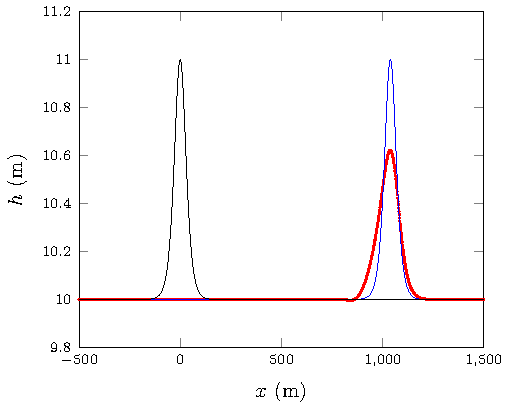
\includegraphics[width=7.0cm]{./results/soliton/ex/newo1-figure0.pdf}}
%\subfigure[][]{\label{fig:solitoneo1u}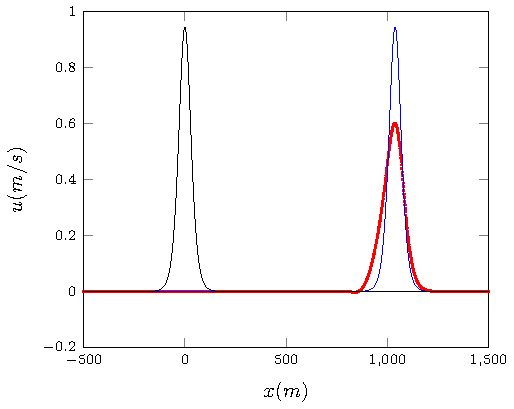
\includegraphics[width=7.0cm]{./results/soliton/ex/newo1u-figure0.pdf}}
%\subfigure[][]{\label{fig:solitoneo2h}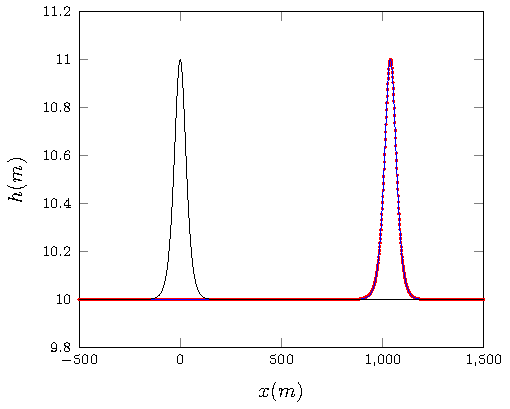
\includegraphics[width=7.0cm]{./results/soliton/ex/newo2-figure0.pdf}}
%\subfigure[][]{\label{fig:solitoneo2u}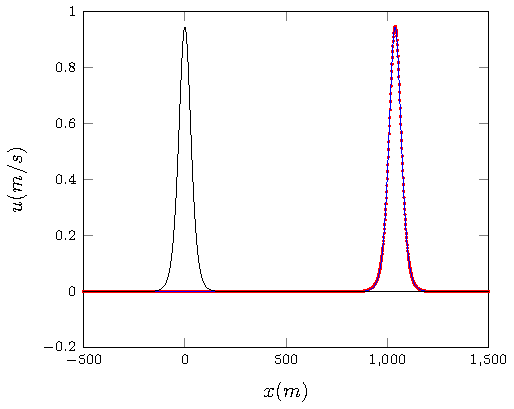
\includegraphics[width=7.0cm]{./results/soliton/ex/newo2u-figure0.pdf}}
%\subfigure[][]{\label{fig:solitoneo3h}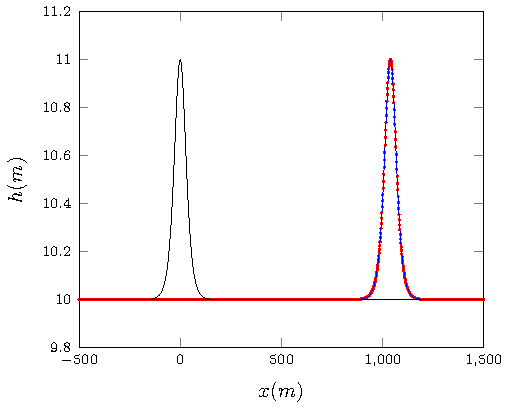
\includegraphics[width=7.0cm]{./results/soliton/ex/newo3-figure0.pdf}}
%\subfigure[][]{\label{fig:solitoneo3u}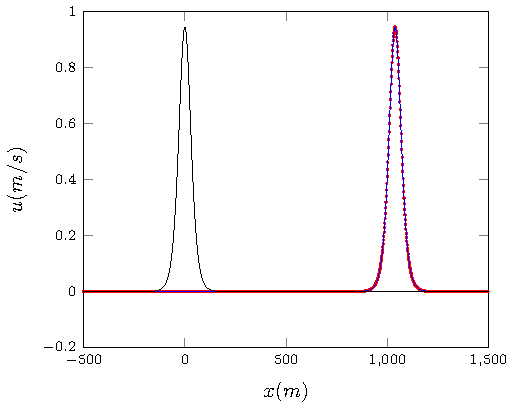
\includegraphics[width=7.0cm]{./results/soliton/ex/newo3u-figure0.pdf}}
%\caption{The first-, second- and third-order simulation of a soliton with $\Delta x = %100 /2^{6}\text{m}$ ($\circ$) plotted against the analytic solution of \eqref{eq:sol} %(\---) with black for $t =0\text{s}$ and blue for $t=100\text{s}$.}
%\label{fig:solitone}
%\end{figure}
%\begin{figure}
%\centering
%\subfigure[][]{\label{fig:solitoncono1}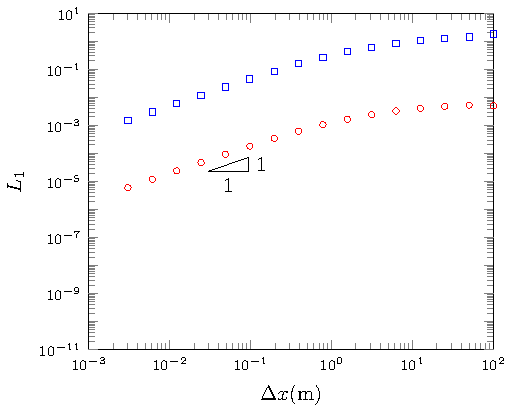
\includegraphics[width=7.0cm]{./results/soliton/con/sto1-figure0.pdf}}
%\subfigure[][]{\label{fig:solitoncono2}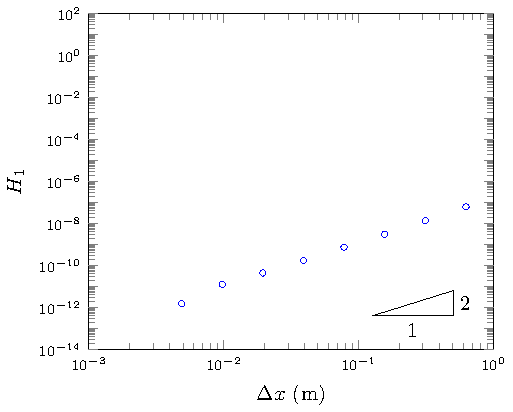
\includegraphics[width=7.0cm]{./results/soliton/con/sto2-figure0.pdf}}
%\subfigure[][]{\label{fig:solitoncono3}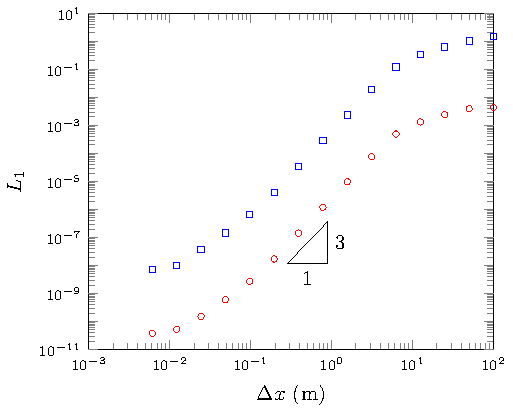
\includegraphics[width=7.0cm]{./results/soliton/con/sto3-figure0.pdf}}
%\caption{Convergence of relative error using $L_1$ norm for analytic soliton solution for both $h$ ($\circ$) and $u$ ($\diamond$) for the; (a) first-, (b) second- and (c) third-order schemes.}
%\label{fig:solitoncon}
%\end{figure} 

%Figure \ref{fig:solitone} demonstrates the superiority of the second- and third-order methods compared to the first-order method. With the first-order method there is significant attenuation of the wave due to its diffusive behaviour which creates a wider wave profile and some smaller trailing waves. However, the first-order method does produce the correct speed of the wave with a small phase error. While the second- and third-order methods demonstrate no noticeable deformation resolving the soliton solution well on a relatively coarse grid with less than $500$ cells defining the actual wave.

%The relative error as measured by the $L_1$-norm of the method can be seen in Figure \ref{fig:solitoncon}. For a vector $\boldsymbol{q}$ and an approximation to it $\boldsymbol{q}^*$ the relative error as measured by the $L_1$-norm is
%\begin{linenomath*}
%\begin{gather*}
%L_1 \left(\boldsymbol{q},\boldsymbol{q}^*\right) = \frac{\sum_{i=1}^{m} |q_i - q^*_i|}{\sum_{i=1}^{m} |q_i|}.
%\end{gather*}
%\end{linenomath*}

%Figure \ref{fig:solitoncon} demonstrates that the schemes all have the correct order of convergence in both time and space. However, this order of convergence is not uniform over all $\Delta x$. When $\Delta x$ is large the actual problem is not discretised well since the cells are too large to adequately resolve the problem; this causes the observed suboptimal rate of convergence in Figure \ref{fig:solitoncon}. When $\Delta x$ is sufficiently small the numerical errors become small enough that floating point errors are significant and this can also lead to suboptimal rates of convergence as can be seen for the third-order method in Figure \ref{fig:solitoncono3}. Therefore, the order of convergence for all methods is confirmed.

%Figure \ref{fig:solitoncon} also demonstrates the superiority of the second- and third-order schemes over the first-order scheme for accuracy. The third-order scheme is also better than the second-order scheme in this respect although this difference is less pronounced. These differences have a significant impact on run-time if one wishes to run a simulation up to a desired accuracy. For instance to run a second- or third-order scheme as accurate as the highest accuracy first-order scheme for $h$ takes significantly less time as can be seen in Table \ref{table:runtime}. This is computationally restrictive 

%Figure \ref{fig:solitoncono2} and Figure \ref{fig:solitoncono3} demonstrate that the second- and third-order schemes both have similar errors and Figure \ref{fig:solitone} shows that these schemes resolve the problem well. Therefore, the extra effort in running a third-order scheme compared to a second-order scheme is not justified in this case. While the effort required to go from a first-order to a second-order scheme is justified since attaining a similar accuracy between them requires a restrictively small $\Delta x$ for a first-order method.   

%--------------------------------------------------------------------------------
\section{Smoothed Dam-Break}
\label{section:smootheddambreak}
%--------------------------------------------------------------------------------
The discontinuous dam-break problem can be approximated by a smooth function using the hyperbolic tan function []. Such an approximation will be called a smoothed dam-break problem and will be defined as such
\begin{linenomath*}
\begin{gather*}
h(x,0) = h_0 + \frac{h_1 - h_0}{2}\left(1 + \tanh\left(a\left(x_0 - x\right)\right)\right),
\end{gather*}
\begin{gather*}
u(x,0) = 0.0m/s.
\end{gather*}
\end{linenomath*}
Where $a$ is given and controls the width of the transition between the two dam-break heights of $h_0$ and $h_1$. For large $a$ the width is small and vice versa. For a fixed $\Delta x$ there are large enough $a$ values such that the transition width is zero. This experiment was run for both of the methods described in this paper and the 3 different order finite difference-volume methods described in []. In this particular simulation $h_0 = 1.0m$, $h_1 = 1.8m$ on $x \in [0m,1000m]$ for $t \in [0s,30s]$ with $x_0 = 500m$. The simulations were run changing both $\Delta x$ and $a$ and for stability $\Delta t = 0.01 \Delta x$ while for the second order finite volume method $\theta = 1.2$.


%--------------------------------------------------------------------------------
\subsection{Changing $a$}
%--------------------------------------------------------------------------------

\begin{figure}
\centering
\subfigure[][]{\label{fig:FDcentdx6normdiff0}\includegraphics[width=7cm]{./results/normaldiff/1dxmdiff/FDcent/6/nb2ne9/0-figure0.pdf}}
\subfigure[][]{\label{fig:FDcentdx6normdiff1}\includegraphics[width=7cm]{./results/normaldiff/1dxmdiff/FDcent/6/nb2ne9/1-figure0.pdf}}
\subfigure[][]{\label{fig:FDcentdx6normdiff2}\includegraphics[width=7cm]{./results/normaldiff/1dxmdiff/FDcent/6/nb2ne9/2-figure0.pdf}}
\subfigure[][]{\label{fig:FDcentdx6normdiff3}\includegraphics[width=7cm]{./results/normaldiff/1dxmdiff/FDcent/6/nb2ne9/3-figure0.pdf}}
\caption{Smooth dam break problem for FDcent [] with $dx = 10 / 2^6 m$ for $a = 0.05$ ($-$ blue), $a = 0.075$ ($-$ green), $a = 0.1$ ($-$ red), $a = 0.25$ ($-$ cyan), $a = 0.5$ ($-$ magenta), $a = 0.75$ ($-$ yellow), $a = 1.00$ ($-$ black)}
\label{fig:FDcentdx6normdiff}
\end{figure}

\begin{figure}
\centering
\subfigure[][]{\label{fig:Grimdx6normdiff0}\includegraphics[width=7cm]{./results/normaldiff/1dxmdiff/grim/6/nb2ne9/0-figure0.pdf}}
\subfigure[][]{\label{fig:Grimdx6normdiff1}\includegraphics[width=7cm]{./results/normaldiff/1dxmdiff/grim/6/nb2ne9/1-figure0.pdf}}
\subfigure[][]{\label{fig:Grimdx6normdiff2}\includegraphics[width=7cm]{./results/normaldiff/1dxmdiff/grim/6/nb2ne9/2-figure0.pdf}}
\subfigure[][]{\label{fig:Grimdx6normdiff3}\includegraphics[width=7cm]{./results/normaldiff/1dxmdiff/grim/6/nb2ne9/3-figure0.pdf}}
\caption{Smooth dam break problem for grim [] with $dx = 10 / 2^6 m$ for $a = 0.05$ ($-$ blue), $a = 0.075$ ($-$ green), $a = 0.1$ ($-$ red), $a = 0.25$ ($-$ cyan), $a = 0.5$ ($-$ magenta), $a = 0.75$ ($-$ yellow), $a = 1.00$ ($-$ black)}
\label{fig:Grimdx6normdiff}
\end{figure}

\begin{figure}
\centering
\subfigure[][]{\label{fig:o1dx6normdiff0}\includegraphics[width=7cm]{./results/normaldiff/1dxmdiff/o1/6/nb6ne13/0-figure0.pdf}}
\subfigure[][]{\label{fig:o1dx6normdiff1}\includegraphics[width=7cm]{./results/normaldiff/1dxmdiff/o1/6/nb6ne13/1-figure0.pdf}}
\subfigure[][]{\label{fig:o1dx6normdiff2}\includegraphics[width=7cm]{./results/normaldiff/1dxmdiff/o1/6/nb6ne13/2-figure0.pdf}}
\subfigure[][]{\label{fig:o1dx6normdiff3}\includegraphics[width=7cm]{./results/normaldiff/1dxmdiff/o1/6/nb6ne13/3-figure0.pdf}}
\caption{Smooth dam break problem for o1 [] with $dx = 10 / 2^6 m$ for $a = 0.5$ ($-$ blue), $a = 0.75$ ($-$ green), $a = 1.0$ ($-$ red), $a = 2.5$ ($-$ cyan), $a = 5.0$ ($-$ magenta), $a = 7.5$ ($-$ yellow), $a = 10.0$ ($-$ black)}
\label{fig:o1dx6normdiff}
\end{figure}

\begin{figure}
\centering
\subfigure[][]{\label{fig:o2dx6normdiff0}\includegraphics[width=7cm]{./results/normaldiff/1dxmdiff/o2/6/nb6ne13/0-figure0.pdf}}
\subfigure[][]{\label{fig:o2dx6normdiff1}\includegraphics[width=7cm]{./results/normaldiff/1dxmdiff/o2/6/nb6ne13/1-figure0.pdf}}
\subfigure[][]{\label{fig:o2dx6normdiff2}\includegraphics[width=7cm]{./results/normaldiff/1dxmdiff/o2/6/nb6ne13/2-figure0.pdf}}
\subfigure[][]{\label{fig:o2dx6normdiff3}\includegraphics[width=7cm]{./results/normaldiff/1dxmdiff/o2/6/nb6ne13/3-figure0.pdf}}
\caption{Smooth dam break problem for o2 [] with $dx = 10 / 2^6 m$ for $a = 0.5$ ($-$ blue), $a = 0.75$ ($-$ green), $a = 1.0$ ($-$ red), $a = 2.5$ ($-$ cyan), $a = 5.0$ ($-$ magenta), $a = 7.5$ ($-$ yellow), $a = 10.0$ ($-$ black)}
\label{fig:o2dx6normdiff}
\end{figure}

\begin{figure}
\centering
\subfigure[][]{\label{fig:o3dx6normdiff0}\includegraphics[width=7cm]{./results/normaldiff/1dxmdiff/o3/6/nb6ne13/0-figure0.pdf}}
\subfigure[][]{\label{fig:o3dx6normdiff1}\includegraphics[width=7cm]{./results/normaldiff/1dxmdiff/o3/6/nb6ne13/1-figure0.pdf}}
\subfigure[][]{\label{fig:o3dx6normdiff2}\includegraphics[width=7cm]{./results/normaldiff/1dxmdiff/o3/6/nb6ne13/2-figure0.pdf}}
\subfigure[][]{\label{fig:o3dx6normdiff3}\includegraphics[width=7cm]{./results/normaldiff/1dxmdiff/o3/6/nb6ne13/3-figure0.pdf}}
\caption{Smooth dam break problem for o3 [] with $dx = 10 / 2^6 m$ for $a = 0.5$ ($-$ blue), $a = 0.75$ ($-$ green), $a = 1.0$ ($-$ red), $a = 2.5$ ($-$ cyan), $a = 5.0$ ($-$ magenta), $a = 7.5$ ($-$ yellow), $a = 10.0$ ($-$ black)}
\label{fig:o3dx6normdiff}
\end{figure}

\begin{figure}
\centering
\subfigure[][]{\label{fig:FDcentdx8normdiff0}\includegraphics[width=7cm]{./results/normaldiff/1dxmdiff/FDcent/8/nb3ne10/0-figure0.pdf}}
\subfigure[][]{\label{fig:FDcentdx8normdiff1}\includegraphics[width=7cm]{./results/normaldiff/1dxmdiff/FDcent/8/nb3ne10/1-figure0.pdf}}
\subfigure[][]{\label{fig:FDcentdx8normdiff2}\includegraphics[width=7cm]{./results/normaldiff/1dxmdiff/FDcent/8/nb3ne10/2-figure0.pdf}}
\subfigure[][]{\label{fig:FDcentdx8normdiff3}\includegraphics[width=7cm]{./results/normaldiff/1dxmdiff/FDcent/8/nb3ne10/3-figure0.pdf}}
\caption{Smooth dam break problem for FDcent [] with $dx = 10 / 2^8 m$ for $a = 0.075$ ($-$ blue), $a = 0.1$ ($-$ green), $a = 0.25$ ($-$ red), $a = 0.5$ ($-$ cyan), $a = 0.75$ ($-$ magenta), $a = 1.0$ ($-$ yellow), $a = 2.5$ ($-$ black)}
\label{fig:FDcentdx8normdiff}
\end{figure}

\begin{figure}
\centering
\subfigure[][]{\label{fig:Grimdx8normdiff0}\includegraphics[width=7cm]{./results/normaldiff/1dxmdiff/grim/8/nb3ne10/0-figure0.pdf}}
\subfigure[][]{\label{fig:Grimdx8normdiff1}\includegraphics[width=7cm]{./results/normaldiff/1dxmdiff/grim/8/nb3ne10/1-figure0.pdf}}
\subfigure[][]{\label{fig:Grimdx8normdiff2}\includegraphics[width=7cm]{./results/normaldiff/1dxmdiff/grim/8/nb3ne10/2-figure0.pdf}}
\subfigure[][]{\label{fig:Grimdx8normdiff3}\includegraphics[width=7cm]{./results/normaldiff/1dxmdiff/grim/8/nb3ne10/3-figure0.pdf}}
\caption{Smooth dam break problem for grim [] with $dx = 10 / 2^8 m$ for $a = 0.075$ ($-$ blue), $a = 0.1$ ($-$ green), $a = 0.25$ ($-$ red), $a = 0.5$ ($-$ cyan), $a = 0.75$ ($-$ magenta), $a = 1.0$ ($-$ yellow), $a = 2.5$ ($-$ black)}
\label{fig:Grimdx8normdiff}
\end{figure}

\begin{figure}
\centering
\subfigure[][]{\label{fig:o1dx8normdiff0}\includegraphics[width=7cm]{./results/normaldiff/1dxmdiff/o1/8/nb6ne13/0-figure0.pdf}}
\subfigure[][]{\label{fig:o1dx8normdiff1}\includegraphics[width=7cm]{./results/normaldiff/1dxmdiff/o1/8/nb6ne13/1-figure0.pdf}}
\subfigure[][]{\label{fig:o1dx8normdiff2}\includegraphics[width=7cm]{./results/normaldiff/1dxmdiff/o1/8/nb6ne13/2-figure0.pdf}}
\subfigure[][]{\label{fig:o1dx8normdiff3}\includegraphics[width=7cm]{./results/normaldiff/1dxmdiff/o1/8/nb6ne13/3-figure0.pdf}}
\caption{Smooth dam break problem for o1 [] with $dx = 10 / 2^8 m$ for $a = 0.5$ ($-$ blue), $a = 0.75$ ($-$ green), $a = 1.0$ ($-$ red), $a = 2.5$ ($-$ cyan), $a = 5.0$ ($-$ magenta), $a = 7.5$ ($-$ yellow), $a = 10.0$ ($-$ black)}
\label{fig:o1dx8normdiff}
\end{figure}

\begin{figure}
\centering
\subfigure[][]{\label{fig:o2dx8normdiff0}\includegraphics[width=7cm]{./results/normaldiff/1dxmdiff/o2/6/nb6ne13/0-figure0.pdf}}
\subfigure[][]{\label{fig:o2dx8normdiff1}\includegraphics[width=7cm]{./results/normaldiff/1dxmdiff/o2/6/nb6ne13/1-figure0.pdf}}
\subfigure[][]{\label{fig:o2dx8normdiff2}\includegraphics[width=7cm]{./results/normaldiff/1dxmdiff/o2/6/nb6ne13/2-figure0.pdf}}
\subfigure[][]{\label{fig:o2dx8normdiff3}\includegraphics[width=7cm]{./results/normaldiff/1dxmdiff/o2/6/nb6ne13/3-figure0.pdf}}
\caption{Smooth dam break problem for o2 [] with $dx = 10 / 2^8 m$ for $a = 0.5$ ($-$ blue), $a = 0.75$ ($-$ green), $a = 1.0$ ($-$ red), $a = 2.5$ ($-$ cyan), $a = 5.0$ ($-$ magenta), $a = 7.5$ ($-$ yellow), $a = 10.0$ ($-$ black)}
\label{fig:o2dx8normdiff}
\end{figure}

\begin{figure}
\centering
\subfigure[][]{\label{fig:o3dx8normdiff0}\includegraphics[width=7cm]{./results/normaldiff/1dxmdiff/o3/6/nb6ne13/0-figure0.pdf}}
\subfigure[][]{\label{fig:o3dx8normdiff1}\includegraphics[width=7cm]{./results/normaldiff/1dxmdiff/o3/6/nb6ne13/1-figure0.pdf}}
\subfigure[][]{\label{fig:o3dx8normdiff2}\includegraphics[width=7cm]{./results/normaldiff/1dxmdiff/o3/6/nb6ne13/2-figure0.pdf}}
\subfigure[][]{\label{fig:o3dx8normdiff3}\includegraphics[width=7cm]{./results/normaldiff/1dxmdiff/o3/6/nb6ne13/3-figure0.pdf}}
\caption{Smooth dam break problem for o3 [] with $dx = 10 / 2^8 m$ for $a = 0.5$ ($-$ blue), $a = 0.75$ ($-$ green), $a = 1.0$ ($-$ red), $a = 2.5$ ($-$ cyan), $a = 5.0$ ($-$ magenta), $a = 7.5$ ($-$ yellow), $a = 10.0$ ($-$ black)}
\label{fig:o3dx6normdiff}
\end{figure}

%--------------------------------------------------------------------------------
\subsection{Changing $dx$}
%--------------------------------------------------------------------------------

%--------------------------------------------------------------------------------
\subsection{Comparison of Models}
%--------------------------------------------------------------------------------

%\subsection{Dam-Break} %old
%--------------------------------------------------------------------------------
%The dam-break problem can be defined as such
%\begin{linenomath*}
%\begin{gather*}
%h(x,0) = \left\lbrace \begin{array}{c c}
%1.8 & x < 500\\
%1.0 & x \ge 500\\
%\end{array} \right. ,
%\end{gather*}
%\begin{gather*}
%u(x,0) = 0.0m/s.
%\end{gather*}
%\end{linenomath*}
%With $x \in \left[0\text{m},1000\text{m}\right]$ for $t \in \left[0\text{s},30\text{s}\right]$. Where $\lambda = 0.01 \text{m/s}$ and $\theta = 1.2$. This corresponds to sub-critical flow and was a situation demonstrated in \citeN{El-etal-2006} and \citeN{Hank-etal-2010-2034}. An example was plotted for %$\Delta x = 100 /2^{10}\text{m}$ for all the methods and for $\Delta x = 100 %/2^{15}\text{m}$ for the first-order method in Figure \ref{fig:DB}. To determine if %the oscillations that occur in the solution indeed converge to some limit as $\Delta x %\rightarrow 0$ multiple $\Delta x$ values were run and then the amount of variation in %the solution measured. This measured how oscillatory the solution was and was used to %determine the growth of the oscillations. A common way to measure this is the total %variation $TV$ \cite{LeVeque-2002} which for $\boldsymbol{q}$ is given by
%\begin{linenomath*}
%\begin{gather*}
%TV(\boldsymbol{q}) = \sum_{\forall i >1} |q_{i} - q_{i-1}|.
%\end{gather*}
%\end{linenomath*}
%If the solution does indeed converge then the TV must at some point plateau, bounding the oscillations. This was indeed the findings of the experiments as can be seen by Figure \ref{fig:DBL1}. The TV increases as $\Delta x$ decreased because the models resolved more dispersive waves. As $\Delta x$ decreased further the TV plateaued and so the size and number of oscillations was bounded. Therefore, the scheme has not become unstable which supports the argument that the numerical schemes do not introduce non-physical oscillations in the solution. The second-order scheme converges rapidly to the solution of the third-order scheme.

%\begin{figure}
%\begin{center}
%\includegraphics[width=8.0cm]{./results/dambreak/L1con/both-figure0.pdf}
%\end{center}
%\caption{The change in total variation (TV) over $\Delta x$ for; ($\circ$) first- , %($\square$) second-, and ($*$) third-order schemes.}
%\label{fig:DBL1}
%\end{figure}
%\begin{figure}
%\centering
%\subfigure[][]{\label{fig:DBo1}\includegraphics[width=7cm]{./results/dambreak/ex/o1-figure0.pdf}}
%\subfigure[][]{\label{fig:DBo2}\includegraphics[width=7cm]{./results/dambreak/ex/o2-figure0.pdf}}
%\subfigure[][]{\label{fig:DBo3}\includegraphics[width=7cm]{./results/dambreak/ex/o3-figure0.pdf}}
%\subfigure[][]{\label{fig:DB1o1}\includegraphics[width=7cm]{./results/dambreak/ex/o1-figure1.pdf}}
%\caption{Solution of the dam-break problem using the (a) first-, (b) second- and (c) third-order method with $\Delta x = 100 /2^{10} \text{m}$. As well as a (d) first-order method with $\Delta x = 100 /2^{15} \text{m}$. }
%\label{fig:DB}
%\end{figure}

%These solutions compare very well to the findings in \citeN{El-etal-2006} with both the second- and third-order schemes resolving the oscillations around the "contact discontinuity"\cite{El-etal-2006} between the rarefaction fan and the shock. In \citeN{Hank-etal-2010-2034} it was reported that for their first-order scheme such oscillatory behaviour was not seen. However, for the first-order scheme proposed in this paper when $\Delta x = 100 /2^{15}$ it was resolved as in Figure \ref{fig:DB1o1}. This validates the findings in \citeN{El-etal-2006}.

%There is also a good agreement between the second- and third-order simulations of the dam-break problem as can be seen in Figures \ref{fig:DBo2} and \ref{fig:DBo3}. Although more oscillations are resolved by the third-order scheme over the second-order scheme, there is no significant change in the resolved behaviour of this problem between the two schemes. As noted in the introduction second-order errors are dissipative; since the diffusive third-order scheme resolved the same oscillations it was demonstrated that none of the dissipative errors significantly polluted the wave train and so the second-order scheme is capable of resolving the problem well.
%--------------------------------------------------------------------------------
\section{Conclusions}
\label{section:Conclusions}
%--------------------------------------------------------------------------------

%--------------------------------------------------------------------------------
\section{Acknowledgements}
%--------------------------------------------------------------------------------

%--------------------------------------------------------------------------------
\bibliography{Serre_ASCE}
%--------------------------------------------------------------------------------

\end{document}
